\documentclass[../main/main.tex]{subfiles}
\begin{document}

%\dominitoc
%\faketableofcontents
\setcounter{chapter}{5}
\chapter{Réponse impulsionnelle de la SEDm}\label{ch:irf}
\minitoc
\vspace{2cm}
Le chapitre précédent était consacré à la modélisation hyperspectrale de
la galaxie hôte en utilisant localement le SED fitter \cigale sur des
images photométrique de PS1. Cette étape d'\hypergal nous fournit le
cube intrinsèque de la galaxie, composé de spaxels ayant chacun un
spectre qui lui est propre.

Les résolutions spectrales et spatiales ne sont cependant pas encore
adaptées à l'espace des observations dans lequel nous souhaitons projeter
le cube, à savoir celui de la SEDm. Nous devons pour cela considérer la
réponse impulsionnelle de notre instrument.

Par ailleurs, l'objectif d'\hypergal étant d'être un modéliseur de
scène, nous serons forcément amenés à modéliser la supernova. Cet objet
étant une source ponctuelle, elle est entièrement définie par le profil
de PSF, qui est la réponse impulsionnelle spatiale de la SEDm.

Dans ce chapitre nous commencerons par présenter la méthode de
détermination de la réponse impulsionnelle spectrale (LSF) de la SEDm,
et son application au cube intrinsèque. Puis nous introduirons un modèle
de profil radial pour la réponse impulsionnelle spatiale, que nous
entraînerons grâce à l'observation d'étoiles standards (sources
ponctuelles). Enfin procéderons à la validation de ce modèle de PSF par
une analyse de la calibration spectrophotométriques à partir de ces
étoiles standards. 
\newpage

\section{Réponse impulsionnelle spectrale: LSF}
% \label{sec:xxx}

\subsection{Lampes à arc}
% \label{ssec:xxx}

Afin de caratériser la réponse impulsionnelle spectrale de la SEDm, nous
utilisons les lampes à arc que nous avons introduit dans le
chapitre~\ref{ssec:wavesol}.

Ces sources de lumière émettent un spectre avec d'intenses raies
d'émissions caractéristiques de l'élément présent dans la lampe.

Nous les utilisons initialement afin de déterminer la solution en longueur
d'onde de chaque trace spectrale sur le CCD, ce qui permet d'associer une longueur d'onde à une localisation spatiale
sur le détecteur du CCD.

Ce processus, détaillé dans \citet{pysedm} et le chapitre~\ref{ch:sedm}
de ce manuscrit, est effectué à l'aide de $3$ lampes à arc: au Xenon (Xe),
Mercure (Hg) et Cadmium (Cd). La combinaison de ces $3$ lampes permet de
couvrir tout le domaine spectral de la SEDm. La
Table~\ref{tab:linearclamp} détaille la position des raies pour chacune
des lampes.

\begin{table}[ht]
  \centerfloat
  \renewcommand{\arraystretch}{1.5}
    \begin{threeparttable}
        \caption{Raies d'émission lampes à arc}
        \label{tab:linearclamp}
        
        \begin{tabular}{lcccccc}
        \toprule
          \textbf{Lampe} &  Raie 1 &  Raie 2 & Raie 3 & Raie 4 & Raie 5 & Raie 6 \\
        \midrule
          \textbf{Hg} & $4047.7$  &  $4359.6$  &  $5462.3$  &  $5781.7^{\star}$  &  \ldots  & \ldots \\
          \textbf{Cd} & $4679.3$  & $4801.3$   & $5087.2$   & $6440.2$ &  \ldots  &  \ldots  \\
          \textbf{Xe} & $7644.1$  & $8250.1^{\star}$  & $8386.2^{\star}$  & $8821.8$  &  $9001.3^{\star}$  &  $9165.1$ \\
          \bottomrule
        \end{tabular}
        \begin{tablenotes}[flushleft]
        \item \textbf{Notes.} La notation $ ^{\star}$ correspond aux
          raies d'emissions qui résultent d'un mélange de plusieurs raies très
          rapprochées spectralement et non disernables par la SEDm.
        \end{tablenotes}
    \end{threeparttable}
  \end{table}

La LSF de la SEDm pouvant très bien être chromatique, nous allons
pouvoir tirer parti de la répartition de ces raies sur toute la plage
spectrale. La Figure~\ref{fig:arclamps} montre le spectre (moyenné sur
tout le MLA) des $3$ lampes à arc utilisées, en unité de flux par
longueur d'onde. La distribution des raies sur l'espace spectral permet
une excellente contrainte entre $4000$ et $6500$\AA\ grâce aux lampes Hg et
Cd. La lampe à Xenon permet, elle, de contraindre la solution en longueur
d'onde (et a fortiori la LSF dans cette étude) au delà de $7500$\AA.


\begin{figure}[ht]
  \centering
  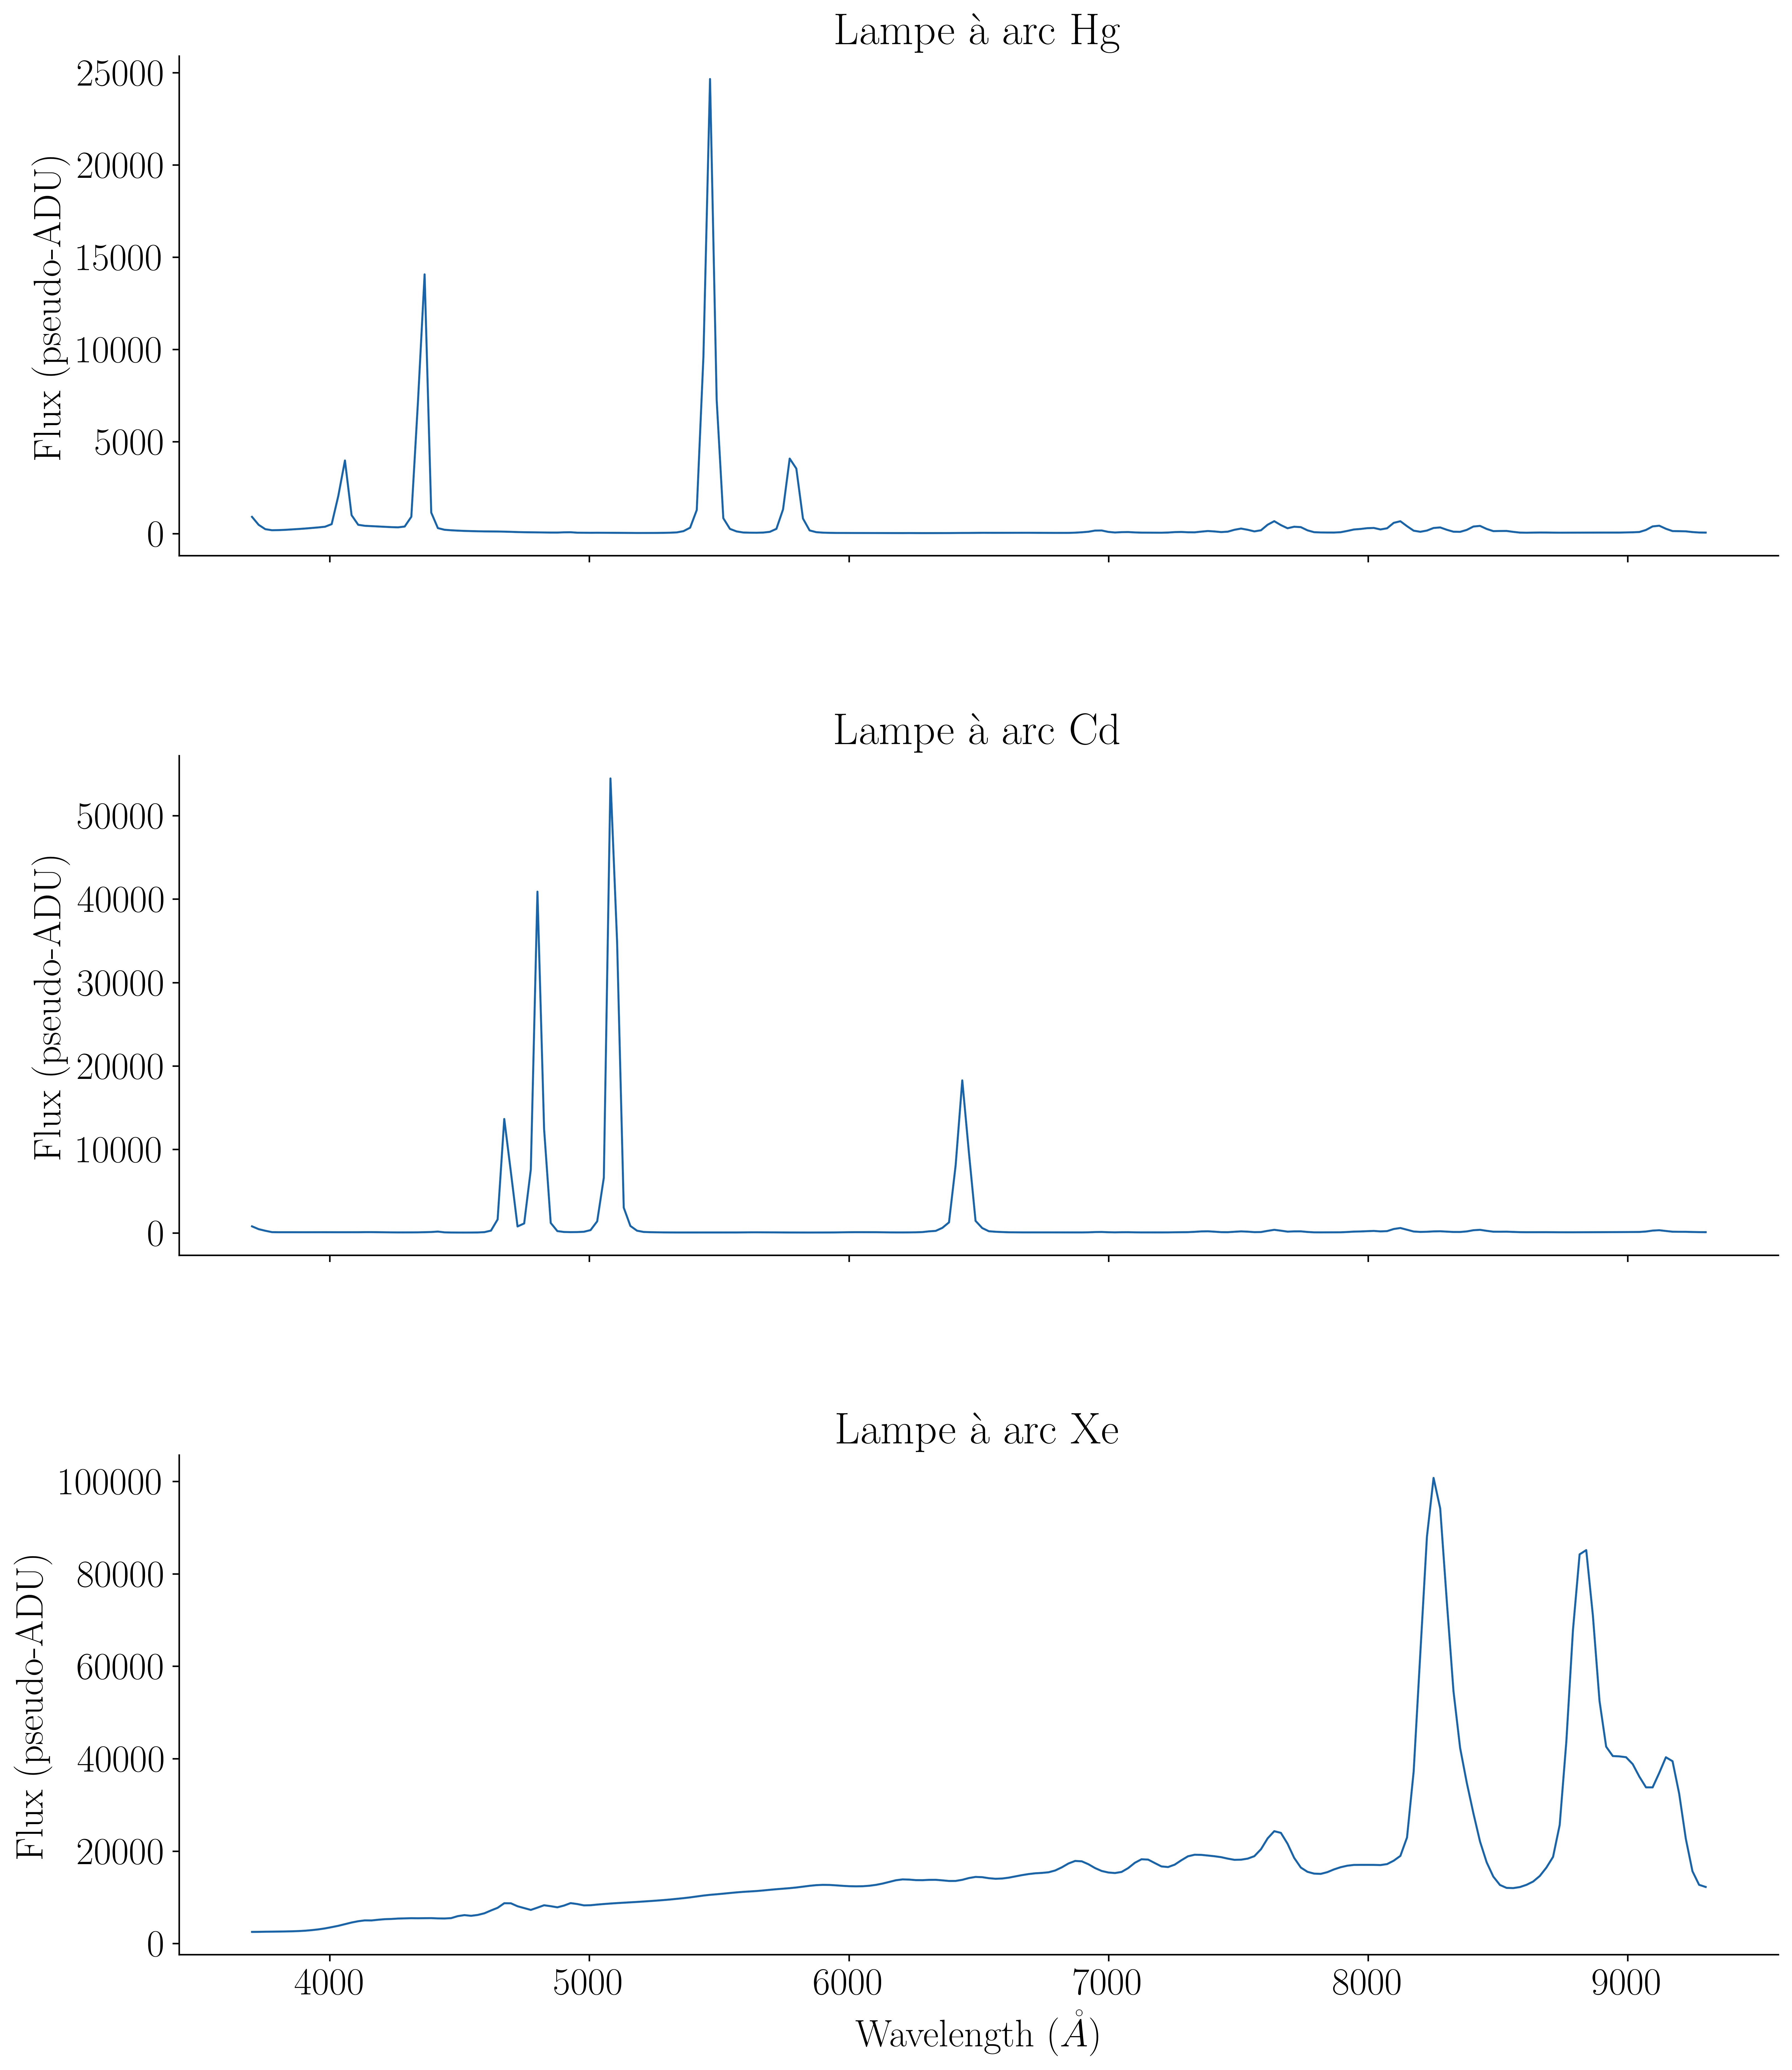
\includegraphics[width=0.99\textwidth]{../figures/06_irf/arclamps.png}
  \caption[Spectres des lampes à arc utilisées pour la SEDm]{Spectres
    des lampes à arc utilisées pour la SEDm pour la nuit du 3 Juillet
    2020. De haut en bas, spectre de la lampe à mercure (Hg), à cadmium
    (Cd) et à Xenon (Xe). Ces spectres sont en unité de flux
    (pseudo-ADU) par longueur d'onde, et sont donc reconstruits à partir
  de la solution en longueur d'onde correspondante. Chaque spectre
  correspond au spectre moyen sur tout le MLA.}
  \label{fig:arclamps}
\end{figure}

\subsection{Détermination de la LSF}
% \label{ssec:xxx}

En toute rigueur, chaque spaxel possède sa propre réponse
impulsionnelle, et il faudrait déterminer la LSF pour chacun d'entre
eux. En pratique, nous faisons la supposition que la LSF moyenne sur
tout le MLA est suffisamment représentative de la réponse impulsionnelle
spectrale de la SEDm à l'échelle locale.

Pour prendre en compte une potentielle variation de la LSF au cours du
temps, nous utilisons les solutions en longueurs d'onde de $65$ nuits
étalées entre 2018 et 2022. Nous récupérons ainsi les positions et
écarts types modélisés pour chaque raie d'émission pour chaque spaxel de
chaque nuit.

Nous utilsons la médiane de la localisation fittée de chaque raie sur tous les
spaxels, de même pour les écarts types, afin d'éviter les potentiels outliers. Les Figure~\ref{fig:lineloc} et
\ref{fig:linestd} montrent la distribution des localisations et écart
types médians des 65 nuits pour chaque raie d'émission. On observe dans
la majorité des solutions en longueur d'onde un biais systématique par
rapport à la longueur d'onde de la raie de référence de l'ordre de
$3$\AA\ pour les lampes Cd et Hg . Les deux dernières raies de Xenon sont très peu contraintes, et
on peut apercevoir une dispersion de l'ordre de $20$\AA\ entre les
différentes nuits d'étude. 

La distribution des écarts types propres à chaque raie indique bien une
évolution chromatique, avec une résolution spectrale plus fine dans le
bleu que dans le rouge. La dispersion sur les nuits sélectionnées est de
l'ordre de quelques \AA.

\begin{figure}[ht]
  \centering
  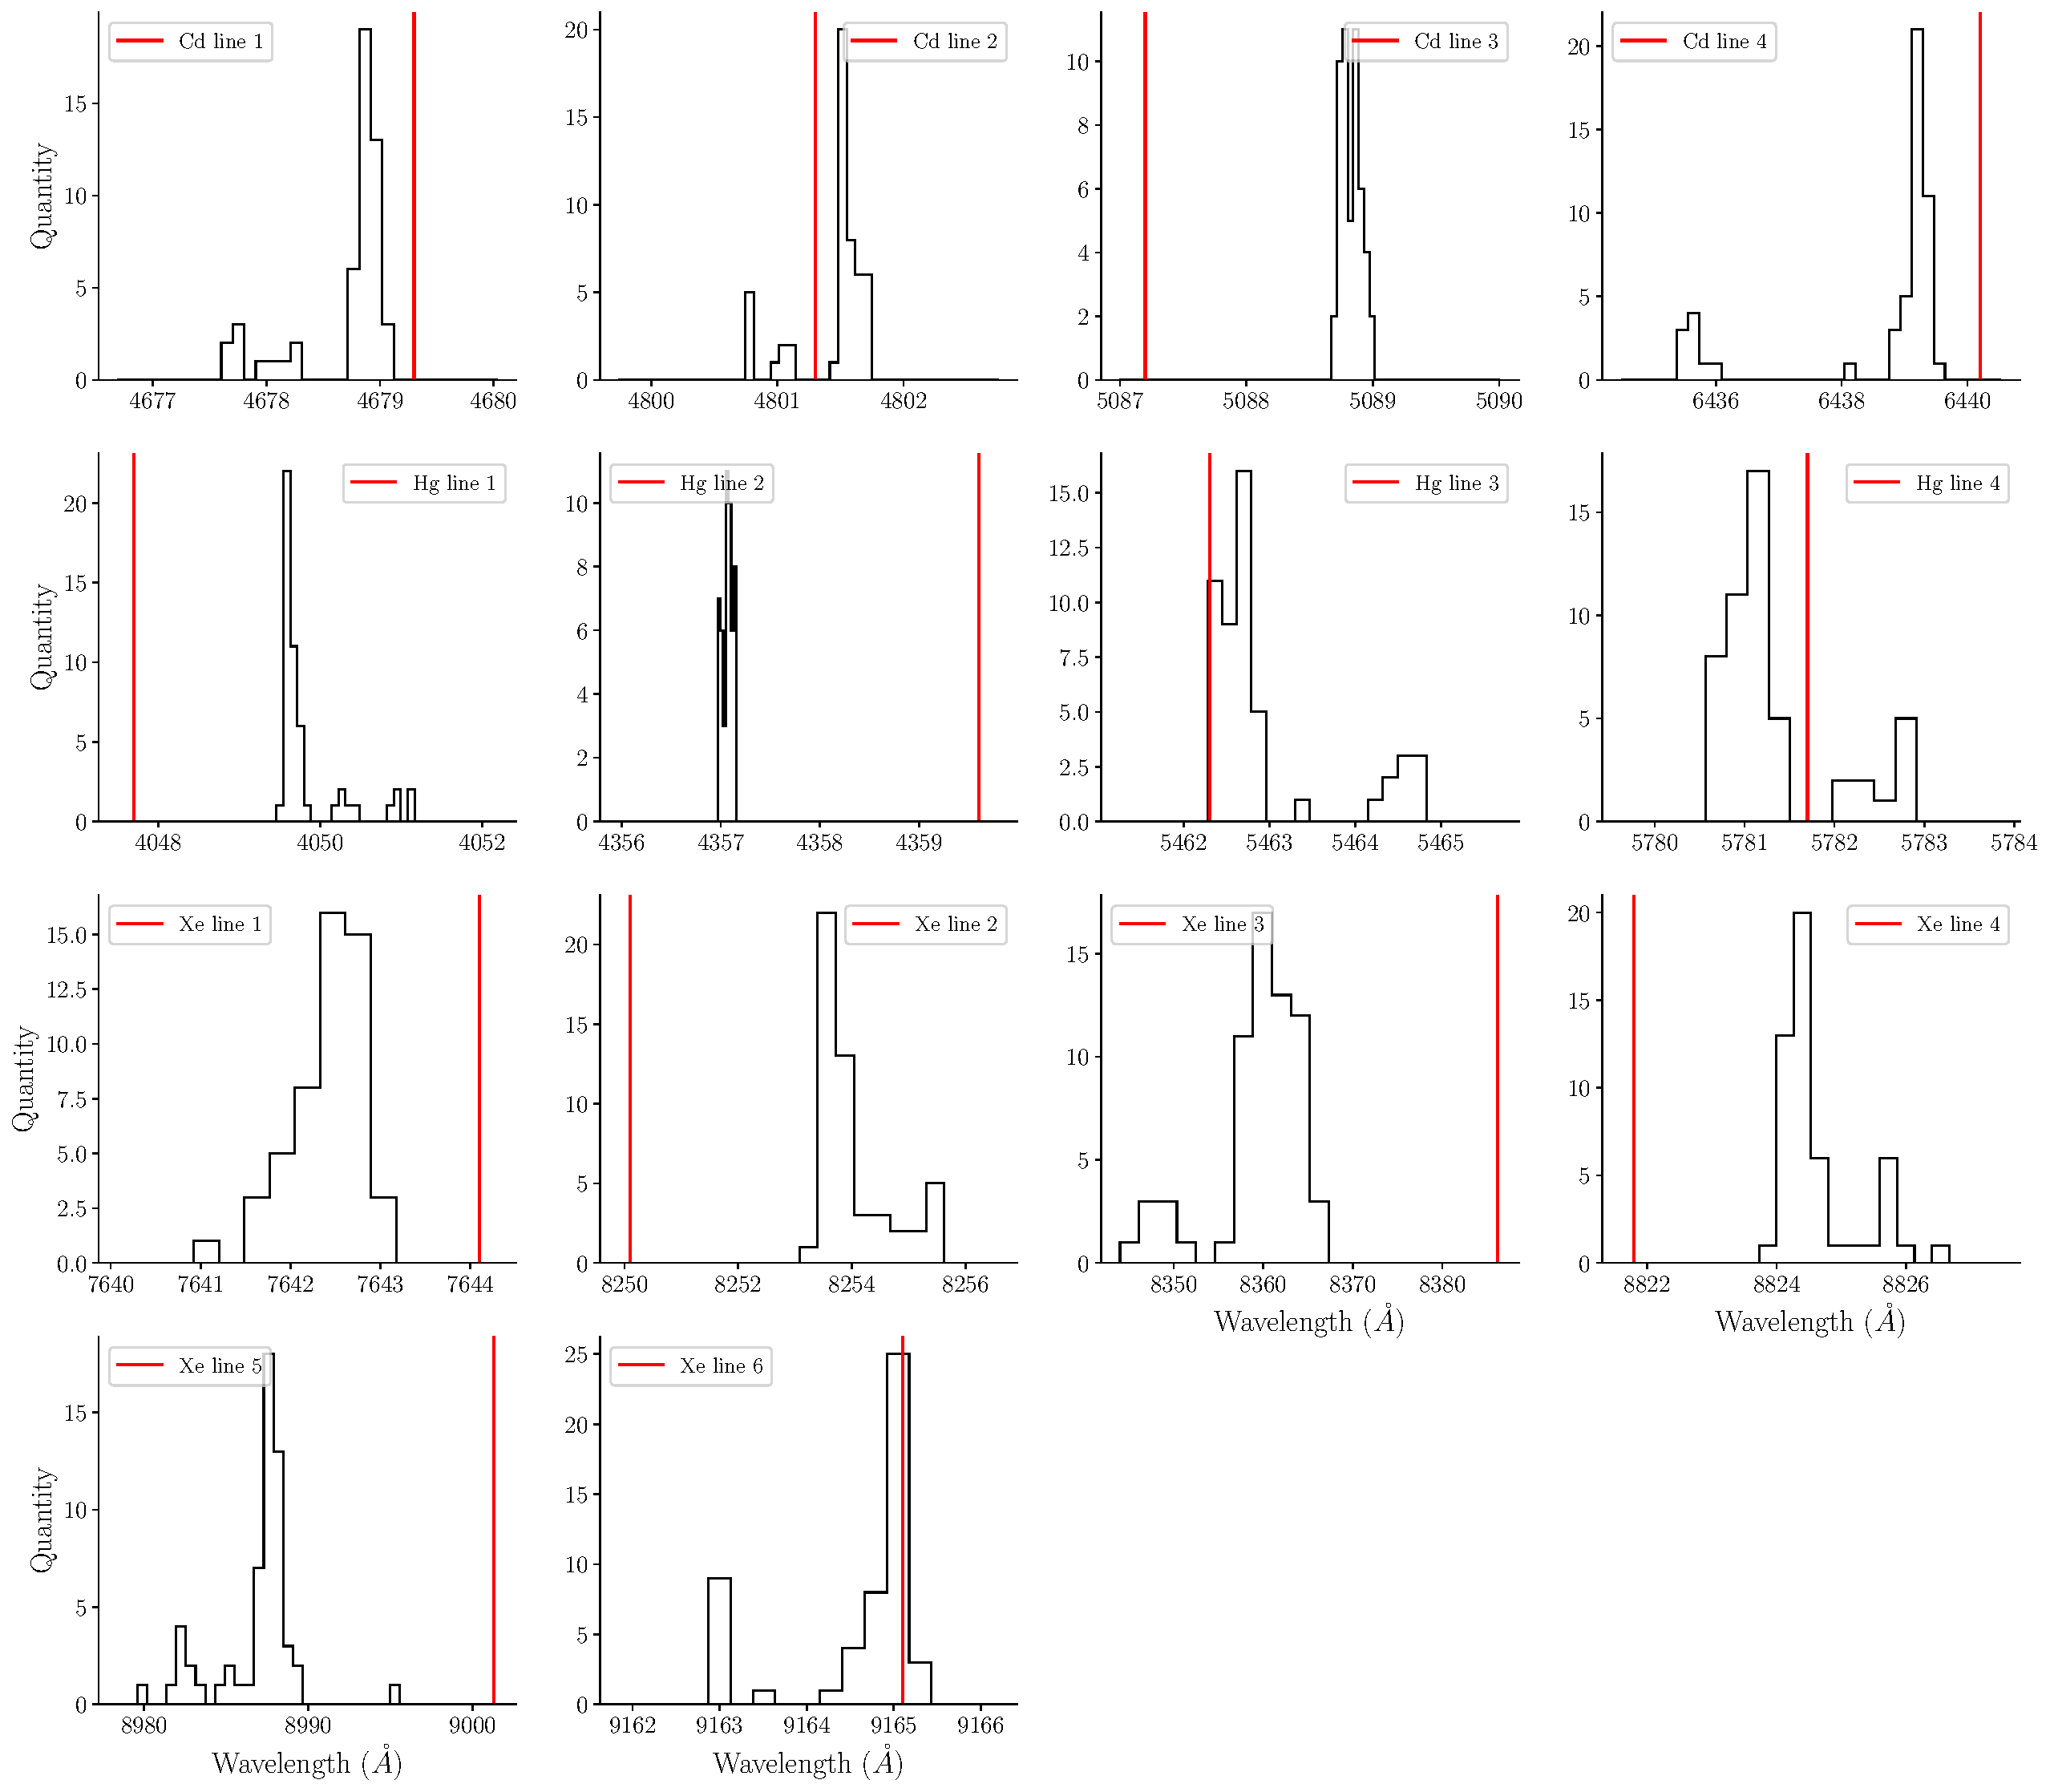
\includegraphics[width=0.99\textwidth]{../figures/06_irf/lineloc.pdf}
  \caption[Distribution de la localisation des raies des lampes à
  arc]{Distribution de la localisation des raies des lampes à arc, en
    considérant la position médiane sur tous les spaxels du MLA pour la
    solution en longueur d'onde de 65 nuits entre 2018 et 2022. La
    localisation rouge verticale indique la position de la raie pour
    chaque lampe suivant les valeurs de la
    Table~\ref{tab:linearclamp}.}
  \label{fig:lineloc}
\end{figure}



\begin{figure}[ht]
  \centering
  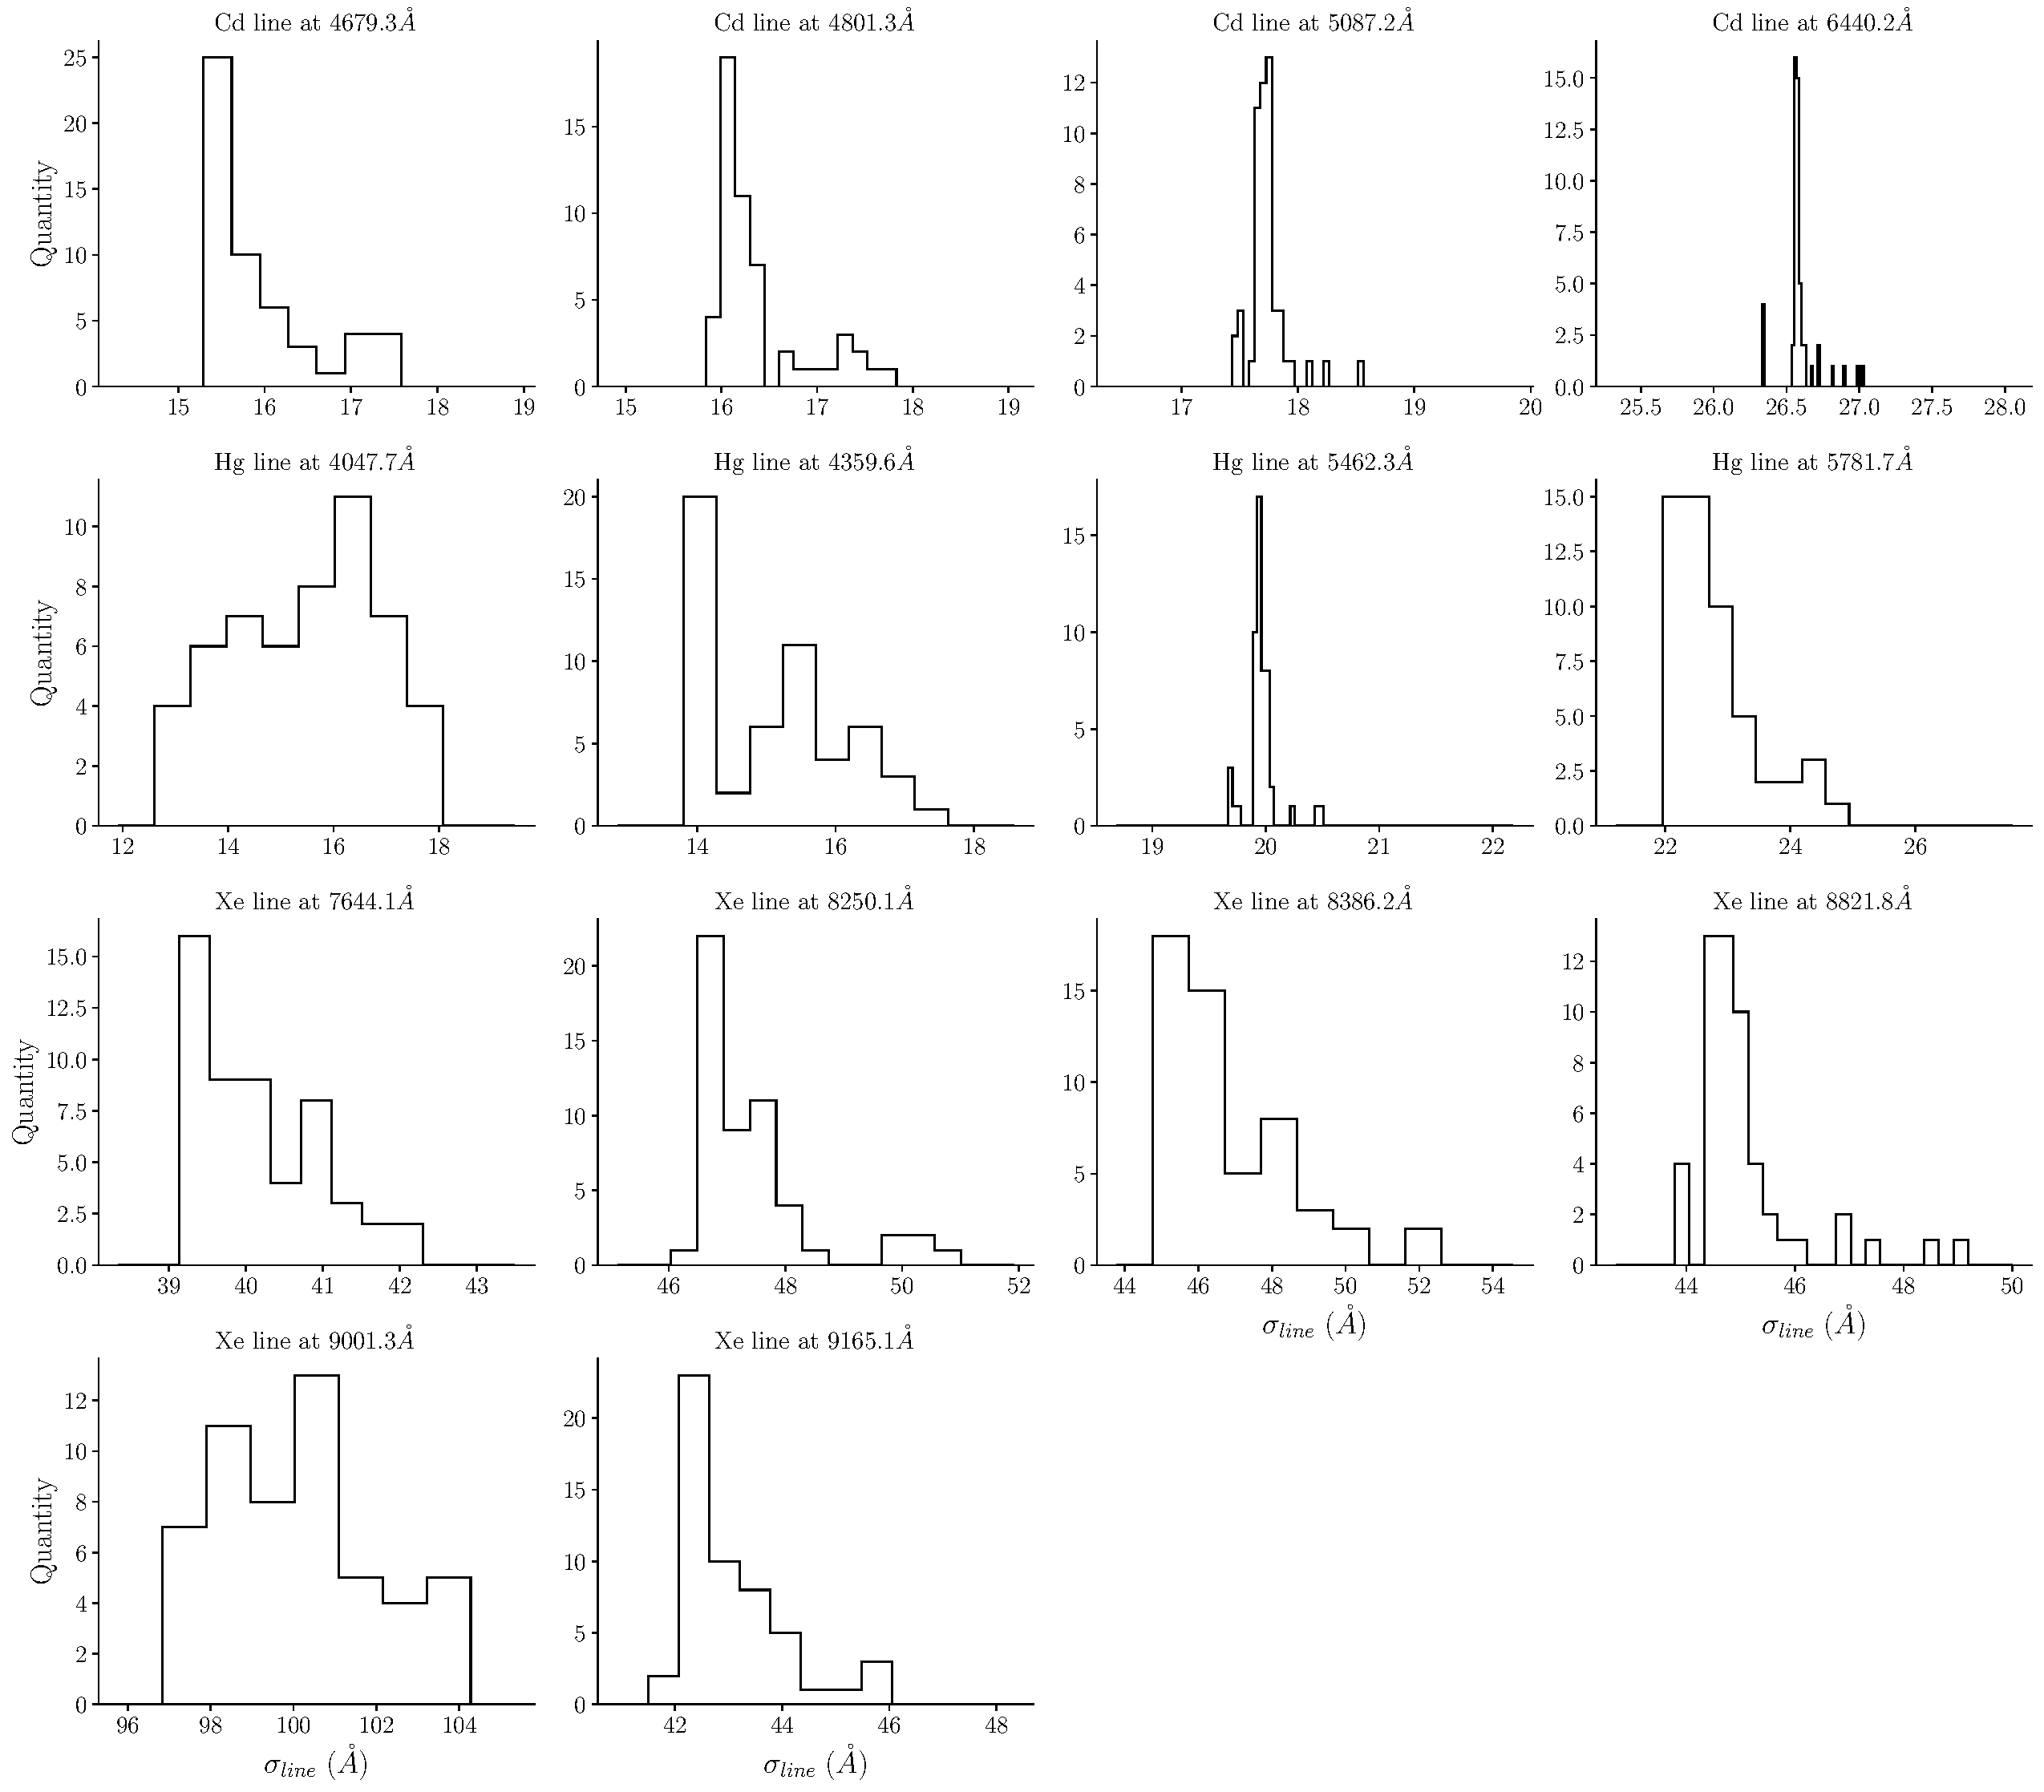
\includegraphics[width=0.99\textwidth]{../figures/06_irf/linestd.pdf}
  \caption[Distribution de l'écart type $\sigma_{line}$ des raies des
  lampes à arc]{Distribution de l'écart type $\sigma_{line}$ des raies
    des lampes à arc, en
    considérant l'écart type médian sur tous les spaxels du MLA pour la
    solution en longueur d'onde de 65 nuits entre 2018 et 2022.}
  \label{fig:linestd}
\end{figure}

Sachant que les raies d'émission de la lampe à Xenon sont faiblement
contraintes, nous choisissons de modéliser la chromaticité de la LSF en
utilisant une combinaison linéaire de polynomes de Legendre de degré 2, afin d'éviter un effet
d'over-fitting aux extrémités.

Pour rappel, les polynômes de Legendre sont
constitués d'une suite de polynômes $p_{n}(x)$ de degré
$n$, et tous les polynômes de la suite sont orthogonaux deux à deux.

On peut les définir sous forme de somme tel que:

\begin{equation}
  \label{eq:legendre}
  P_{n}(x)=\frac{1}{2^{n}}\sum^{n}_{k=0}\binom{n}{k}^{2}(x-1)^{n-k}(x+1)^{k}
\end{equation} 

Nous montrons dans la Figure~\ref{fig:lsf} la modélisation de la LSF
chromatique, avec les coefficients fittés des polynomes de Legendre
étant:
\begin{align*}
  C_{0}&=19.65\pm 0.32\\
  C_{1}&=26.0\pm 0.6\\
  C_{2}&=7.3\pm 0.6
\end{align*}

\begin{figure}[ht]
  \centering
  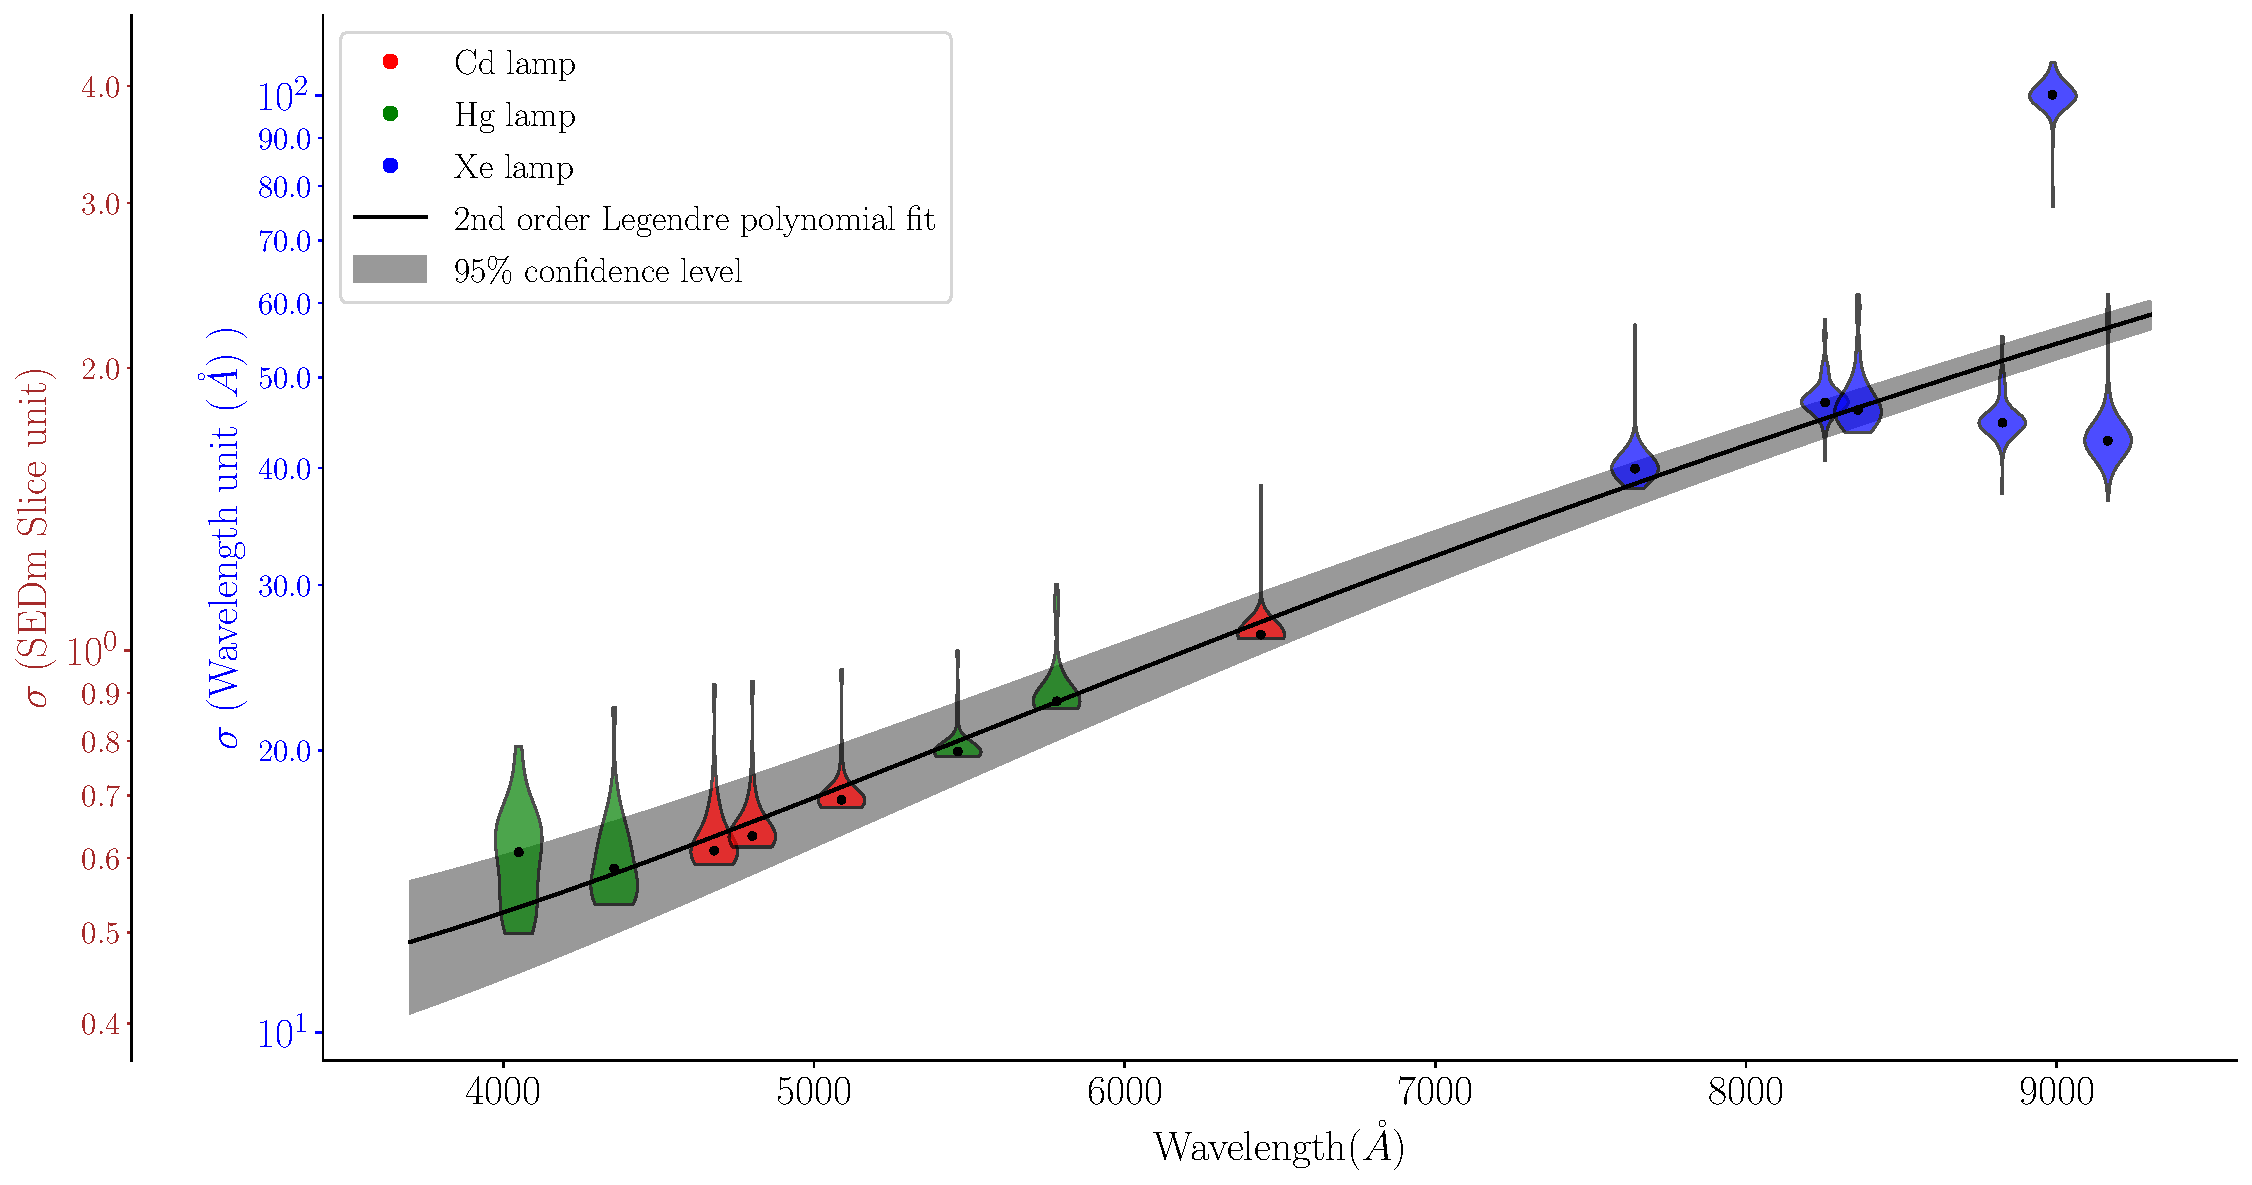
\includegraphics[width=0.99\textwidth]{../figures/06_irf/LSF.pdf}
  \caption[Chromaticité de la LSF]{Chromaticité de la LSF}
  \label{fig:lsf}
\end{figure}

\section{Réponse impulsionnelle spatiale: PSF}
%\label{ssec:xxx}

\subsection{Modèle de profil radial}
%\label{ssec:xxx}

\subsection{Entrainement du modèle}

\subsection{Chromaticité et ADR}\label{ssec:chromadr}

\section{Validation}
%\label{sec:xxx}

\subsection{Calibration photométrique}
%\label{ssec:xxx}

\subsection{Résultats}
%\label{ssec:xxx}


%\bibliographystyle{../main/aa_url2}
%\bibliography{99_references}

\end{document}

%%% Local Variables:
%%% mode: latex
%%% TeX-master: t
%%% End:
